\documentclass[11pt,a4paper]{article}
\usepackage[margin=2.2cm]{geometry}
\usepackage{graphicx,booktabs,amsmath,amssymb,hyperref,xcolor,enumitem,caption,float}
\hypersetup{colorlinks=true,linkcolor=blue!50!black,urlcolor=blue!50!black,citecolor=blue!50!black}
\setlist{nosep,leftmargin=*}
\captionsetup{font=small,labelfont=bf}
\graphicspath{{../results/}}
\newcommand{\NImages}{5,775}
\newcommand{\NMorph}{33}
\newcommand{\NWells}{3,300}
\newcommand{\NSCfusion}{85.4\%}
\newcommand{\NSCBfusion}{77.2\%}
\newcommand{\NSCcell}{85.4\%}
\newcommand{\NSCBcell}{80.4\%}
\newcommand{\NSCfield}{79.6\%}
\newcommand{\NSCBfield}{71.7\%}
\newcommand{\NSCclassical}{70.9\%}
\newcommand{\NSCBclassical}{59.8\%}
\newcommand{\NSCnotvn}{79.6\%}
\newcommand{\NSCBnotvn}{67.4\%}
\newcommand{\NSCbalfusion}{84.6\%}
\newcommand{\CovNinety}{91.3\%}
\newcommand{\SizeNinety}{1.18}
\newcommand{\SingNinety}{83.5\%}
\newcommand{\CovNinetyFive}{96.1\%}
\newcommand{\SizeNinetyFive}{1.73}
\newcommand{\CovEighty}{85.4\%}
\newcommand{\SizeEighty}{1.00}
\newcommand{\SensFusMin}{84.5\%}
\newcommand{\SensFusMax}{88.3\%}
\newcommand{\SensNSCmin}{78.6\%}
\newcommand{\SensNSCmax}{90.3\%}
\newcommand{\SensNSCmed}{85.4\%}
\newcommand{\SensNSCBmin}{70.7\%}
\newcommand{\SensNSCBmax}{83.7\%}
\newcommand{\SensNSCBmed}{79.3\%}
\newcommand{\NoveltyAUROC}{0.79}
\newcommand{\PctReplicating}{37.3\%}
\newcommand{\PctReplicatingAnn}{88.3\%}
\newcommand{\NCompounds}{112}
\newcommand{\NInactive}{24}
\newcommand{\NToxOnly}{14}
\newcommand{\NNonTox}{11}
\newcommand{\NWideWindow}{7}
\newcommand{\NNarrow}{21}
\newcommand{\NToxFirst}{35}

% ---- fill in -------------------------------------------------------------
\newcommand{\repo}{\url{https://github.com/shreshth006/shennongs-glass}}
\newcommand{\TeamName}{Shreshth Mishra}
\newcommand{\TeamDetails}{Solo entry: Shreshth Mishra (team leader; AI / computer science). Kaggle: aerochrome.}
% --------------------------------------------------------------------------

\title{\textbf{Shennong's Glass}: training-free foundation-model phenotypic screening\\
with calibrated uncertainty for organ-on-chip drug evaluation}
\author{\TeamName --- AI4S Open Innovation: AI for Life Science\\[2pt]
\small Category: \textbf{End-to-End System} \quad$\cdot$\quad Code: \repo}
\date{October 2026}

\begin{document}
\maketitle

\begin{abstract}
Organ-on-chip (OoC) and other microphysiological systems produce rich imaging read-outs, but
turning those images into decisions --- \emph{is this compound active, how does it act, at what
dose does it become toxic, and can I trust the call?} --- still depends on hand-tuned image
analysis and expert inspection. We present \textbf{Shennong's Glass}, an end-to-end system that takes
standard three-channel endpoint stains (nuclei, $\beta$-tubulin, F-actin) and returns (i) a
phenotypic activity score calibrated against vehicle controls, (ii) a viability read-out and
Hill-fitted dose--response, (iii) a mechanism-of-action (MoA) ranking with a
\emph{conformal prediction set} of guaranteed coverage, (iv) a novel-mechanism alarm and (v) a
plain-language explanation of what changed in the cells. The image encoder is a frozen
self-supervised foundation model (DINOv2), so no task-specific training or labels are needed and
the system transfers to a new chip by swapping its reference library. On the BBBC021 benchmark
(\NImages{} fields, 113 compounds, 8 doses each) Shennong's Glass reaches \NSCfusion{} MoA accuracy on
held-out compounds (NSC) and \NSCBfusion{} when also holding out imaging batches (NSCB);
its 90\% conformal sets achieve \CovNinety{} empirical coverage with \SizeNinety{} classes on
average, and it flags mechanisms absent from its library with AUROC \NoveltyAUROC. Across
\NCompounds{} compounds it separates phenotypic potency from cytotoxicity and triages compounds by
the width of that window. Everything --- features, figures and the interactive demo --- is
reproducible with free Kaggle notebooks and a laptop CPU.
\end{abstract}

\begin{quote}\small\itshape
Shennong, the Divine Farmer of Chinese legend, tasted hundreds of herbs to tell medicine from
poison; his body, the story goes, was transparent, so that he could watch each herb act on his
organs. An organ-on-chip is that transparent body. Shennong's Glass is the eye that watches it.
\end{quote}

\section{Problem and application scenario}
OoC platforms recapitulate tissue-level physiology and are increasingly used for efficacy and
toxicity testing before animal or human studies~\cite{ingber2022,low2021}. Their most common
quantitative endpoint is still fluorescence imaging of fixed tissue: nuclei (DAPI/Hoechst) for
cell number and nuclear state, and cytoskeletal stains --- $\beta$-tubulin and F-actin --- for cell
shape, neurite/axon integrity and barrier morphology. Neural OoC platforms such as those of the
challenge supporter rely on exactly these markers, since microtubule integrity is what
chemotherapy-induced peripheral neuropathy destroys~\cite{staff2017}.

Three practical gaps limit how much value is extracted from such images:
\begin{enumerate}
\item \textbf{Analysis is assay-specific.} Pipelines are tuned per cell type and per question,
and deep models trained on one assay rarely transfer; OoC datasets are too small to train them.
\item \textbf{Calls come without reliability.} A classifier always outputs \emph{some} MoA, even
for an inactive compound or a mechanism it has never seen; a screening scientist needs to know
when not to trust it.
\item \textbf{Potency and toxicity are judged separately.} A morphological effect is only
interesting if it appears at doses below overt cytotoxicity.
\end{enumerate}
Shennong's Glass addresses all three in one system, and presents the result in an interface a biologist
can use without writing code (Section~\ref{sec:demo}).

\section{Data, licences and compliance}
\paragraph{BBBC021v1}~\cite{caie2010,ljosa2012}: MCF-7 breast-cancer cells treated for 24\,h with
113 small molecules at 8 concentrations (plus DMSO vehicle and positive controls), imaged in
three channels (DAPI, $\beta$-tubulin, F-actin) at 4 fields per well on 55 plates in 10 weekly
batches; 13{,}200 fields in total. A curated subset of 103 compound--concentration
\emph{treatments} (38 compounds) is annotated with one of 12 MoAs. We used
fields of view 1 and 3 of every well (\NImages{} fields, \NWells{} wells; Section~\ref{sec:limits}).
Images and labels are copyright AstraZeneca and distributed for research by the Broad Bioimage
Benchmark Collection; we do not redistribute them --- our scripts fetch them from the public
sources. The dataset contains no human or patient data.
\paragraph{Models and libraries.} DINOv2 ViT~\cite{oquab2023} (Apache-2.0), PyTorch, scikit-image,
scikit-learn, UMAP, Gradio (all open-source licences). No commercial API is used.

\section{Method}
\begin{figure}[t]
\centering
\fbox{\begin{minipage}{0.96\linewidth}\small\centering
\textbf{3-channel field} $\rightarrow$
\textbf{(a)} nuclei segmentation (Otsu + distance-transform watershed) $\rightarrow$ cell territories $\rightarrow$ \NMorph{} interpretable features\\[2pt]
\textbf{(b)} single-cell crops $\rightarrow$ frozen DINOv2 per channel $\rightarrow$ mean cell embedding
\quad \textbf{(c)} whole field $\rightarrow$ frozen DINOv2 per channel\\[4pt]
$\downarrow$ per-plate DMSO centring + typical-variation normalisation (PCA whitening on DMSO wells)\\[2pt]
$\downarrow$ well profile $\rightarrow$ treatment profile (median of replicates) $\rightarrow$ fusion of (a)+(b)+(c)\\[4pt]
\textbf{MoA 1-NN} $\cdot$ \textbf{conformal set} $\cdot$ \textbf{novelty flag} $\cdot$
\textbf{dose--response \& cytotoxicity window} $\cdot$ \textbf{plain-language explanation}
\end{minipage}}
\caption{Shennong's Glass pipeline. No component is trained on BBBC021 labels.}
\label{fig:pipeline}
\end{figure}

\subsection{Three complementary views of each field}
\textbf{(a) Interpretable morphology.} Nuclei are segmented on the DAPI channel at half resolution
(Gaussian smoothing, Otsu threshold, distance-transform watershed); each nucleus is grown by up to
20\,px into the cytoskeletal foreground to approximate its cell. Per cell we measure nuclear area,
perimeter, eccentricity, solidity, axis lengths, DNA intensity and integrated DNA content, cell
area, tubulin and actin intensities, cytoplasm-to-nucleus ratio and cell elongation, and per field
the cell count, channel coverage and edge-texture of each channel. Fields are summarised by the
median and inter-quartile range across cells (\NMorph{} features). These features carry the
explanations shown to users and double as a classical baseline.

\textbf{(b) Single-cell foundation-model embedding.} Around a random subset of segmented nuclei we
cut fixed-size crops (one cell plus its immediate neighbourhood). Each channel is embedded
separately by a frozen DINOv2 ViT (grey-scale replicated to RGB, ImageNet normalisation) and the
class tokens are averaged over cells, then concatenated across channels. Embedding channels
separately avoids imposing a false RGB semantics on fluorescence stains and keeps the method
applicable to any number of channels.

\textbf{(c) Whole-field embedding.} The full field is embedded per channel (class token and mean
patch token), capturing tissue-level context --- density, clustering, debris --- that single-cell
crops miss.

\subsection{Normalisation anchored on vehicle controls}
Plate and batch effects dominate raw image features. For every plate we subtract the mean of its
DMSO wells; we then fit a PCA on DMSO wells only and whiten (typical variation normalisation,
TVN~\cite{ando2017}), so that the remaining axes describe drug-induced rather than nuisance
variation. Classical features are robust-$z$-scored against the plate's DMSO median and pooled
DMSO MAD. Fields are averaged into wells and wells into treatments (median over replicates). The
fusion profile concatenates the $\ell_2$-normalised blocks (b), (c) and (a) (weight 0.7).

\subsection{Mechanism of action and calibrated uncertainty}
\textbf{MoA ranking.} A query profile is compared by cosine similarity to the reference
treatments; the score of a MoA is the similarity to its closest reference, turned into
probabilities with a temperature softmax. This nearest-neighbour design needs no training, makes
every call traceable to concrete reference compounds (shown in the app) and lets users add new
references instantly.

\textbf{Conformal prediction sets.} Instead of a single label Shennong's Glass reports the smallest set
of MoAs that contains the truth with user-chosen probability $1-\alpha$. We use split-conformal
prediction~\cite{vovk2005,angelopoulos2021} with non-conformity $1-\hat p(\text{true MoA})$
calibrated \emph{leave-one-compound-out}: for each query compound the threshold is computed on all
other compounds only. Under exchangeability of compounds this guarantees marginal coverage
$\geq 1-\alpha$ on new compounds; large sets honestly signal ambiguity.

\textbf{Novel-mechanism detection.} If the maximum similarity to the library falls below the 5th
percentile observed for in-library compounds, the call is flagged as a possible new mechanism. We
evaluate this by hiding each query's own MoA from the library.

\subsection{Dose--response, cytotoxicity and triage}
\textbf{Viability} of a well is its cell count relative to the median DMSO well on the same plate.
\textbf{Phenotypic activity} is the distance of the well's single-cell profile from the DMSO
centre in whitened space; its null distribution is given by the DMSO wells themselves, and a well
is called active above the 99th percentile of that null (1\% false-positive rate on vehicle);
a compound is active from the lowest dose at which this holds for that dose \emph{and} the next
higher one, which controls false positives across the eight-dose series.
Both read-outs are fitted with four-parameter Hill curves on $\log_{10}$ concentration. From the
dose series we derive the lowest active and lowest cytotoxic (viability $<50\%$) concentrations,
their ratio --- the \emph{phenotype-to-cytotoxicity window} --- and a triage label:
inactive; cytotoxic without a distinct phenotype; active and non-cytotoxic; active
$\geq10\times$ below cytotoxicity; narrow window; phenotype only at cytotoxic doses.

\subsection{Explanations}
For every MoA we report its median morphological signature (Fig.~\ref{fig:sig}); for every query,
the classical features deviating most from DMSO are rendered as sentences (e.g.\ ``nuclear area
increased (+3.1\,SD vs.\ DMSO)'').

\section{Implementation}
Feature extraction (\texttt{kaggle/features/features.py}) runs as Kaggle notebooks over the public
BBBC021 mirror; analysis (\texttt{scripts/run\_analysis.py}, $<1$ min on a laptop CPU) produces
all numbers and figures in this report from the extracted features; numbers in the text are
inserted automatically from \texttt{results/metrics.json}. The demo (\texttt{app/app.py}, Gradio)
reuses the identical extraction code (\texttt{shennong/extract.py}) on uploaded images. The
configuration used for the reported results is a DINOv2 ViT-S/14, 16 single-cell crops per field
($128\times128$\,px, embedded at $112\times112$) and fields embedded at $224\times280$; the
extraction script also supports ViT-B/14 at higher resolution for GPU runs.

\section{Experiments and results}
\subsection{Mechanism-of-action benchmark}
We follow the standard protocol~\cite{ljosa2013}: 1-nearest-neighbour MoA assignment of the 103
annotated treatments, never matching a treatment to another dose of the same compound
(\emph{not-same-compound}, NSC). The stricter NSCB additionally forbids matches to treatments
imaged in the same batch and, as is customary, drops the two MoAs that occur in a single batch
(92 treatments).

\begin{table}[H]
\centering\small
\begin{tabular}{lcc}
\toprule
Profile & NSC & NSCB \\
\midrule
Classical morphology (\NMorph{} interpretable features) & \NSCclassical & \NSCBclassical \\
DINOv2 single cells, plate-centred only (no TVN) & \NSCnotvn & \NSCBnotvn \\
DINOv2 whole field + TVN & \NSCfield & \NSCBfield \\
DINOv2 single cells + TVN & \NSCcell & \NSCBcell \\
\textbf{Fusion (Shennong's Glass)} & \textbf{\NSCfusion} & \textbf{\NSCBfusion} \\
\bottomrule
\end{tabular}
\caption{1-NN MoA accuracy on held-out compounds (main configuration). For context, the best
published pipelines on this benchmark --- hand-engineered CellProfiler profiles with factor
analysis, or deep networks trained on BBBC021 --- report roughly 90--96\% NSC~\cite{ljosa2013,ando2017}.
Our training-free, reduced-compute configuration is below that range; its value lies in needing
no labelled training data, in its calibrated uncertainty (Section~\ref{sec:rel}) and in its stability
across design choices (Table~\ref{tab:sens}).}
\label{tab:bench}
\end{table}

\begin{figure}[H]
\centering
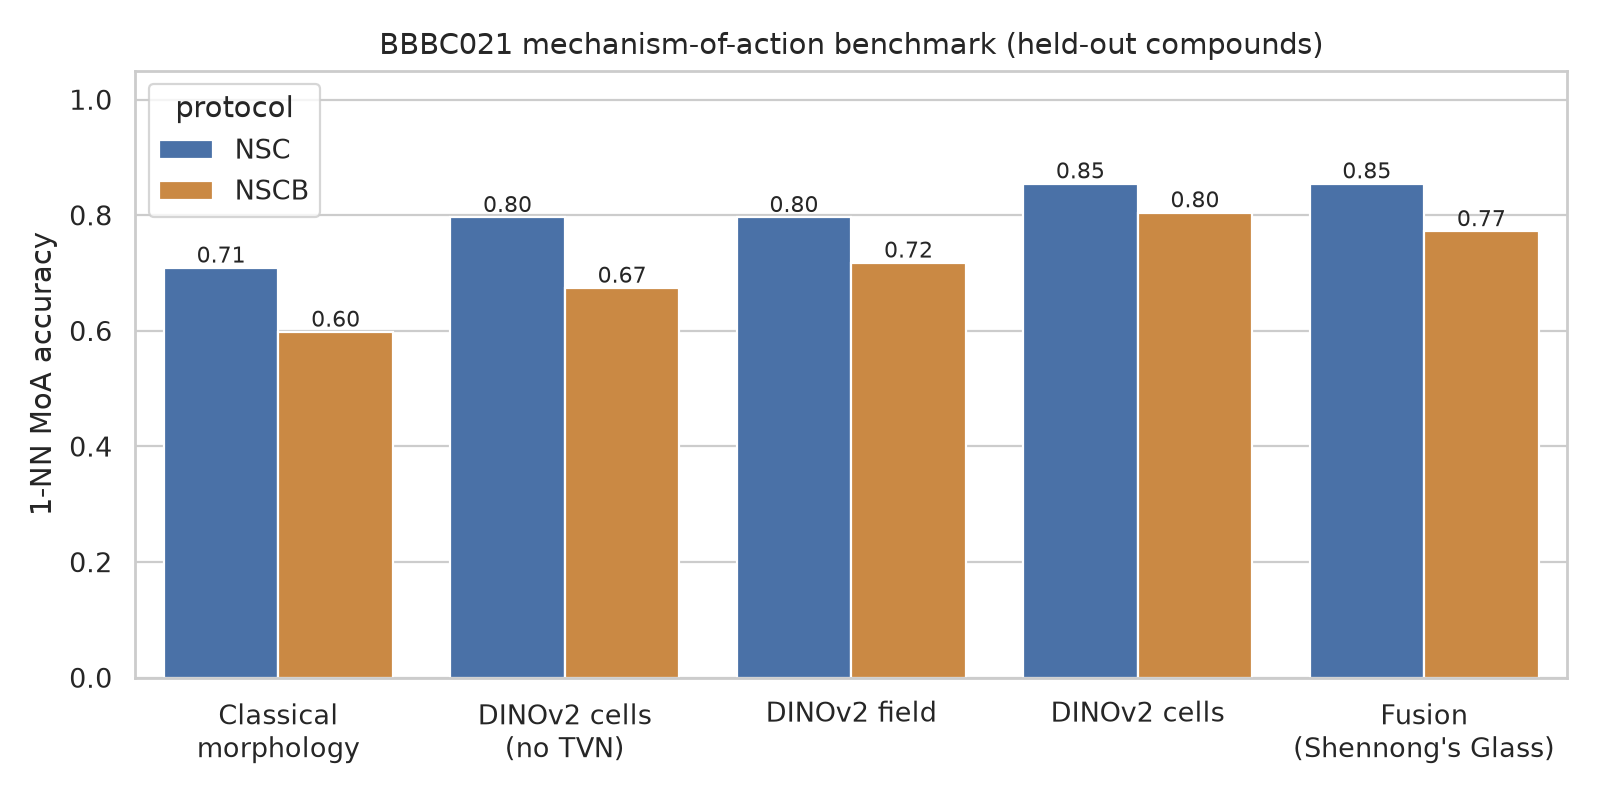
\includegraphics[width=0.78\linewidth]{fig_benchmark.png}
\caption{MoA accuracy by profile type and protocol.}
\end{figure}

\paragraph{Robustness to design choices.} The main configuration (128 TVN components,
classical-block weight 0.7) was fixed in code before any result was computed. Because 103
treatments make each percentage point roughly one treatment, Table~\ref{tab:sens} reports the
benchmark across the alternatives we considered rather than the best one. Single views move
substantially with the number of whitening components (\SensNSCmin--\SensNSCmax{} NSC over the
whole grid), whereas the fused profile stays within \SensFusMin--\SensFusMax{} NSC in every setting:
combining views mainly buys \emph{stability}. Full-rank whitening (330 components, one per
DMSO well) was also tested and is worse (82.5\% NSC), as expected when the vehicle covariance is
estimated from as many wells as dimensions.

\begin{table}[H]
\centering\small
\begin{tabular}{lcccc}
\toprule
Profile & TVN 32 & TVN 64 & TVN 128 & TVN 256 \\
\midrule
cells & 82.5 / 70.7 & 79.6 / 73.9 & 85.4 / 80.4 & 90.3 / 83.7 \\
field & 84.5 / 79.3 & 81.6 / 79.3 & 79.6 / 71.7 & 78.6 / 73.9 \\
cells+field & 87.4 / 81.5 & 86.4 / 80.4 & 82.5 / 79.3 & 89.3 / 81.5 \\
fusion (w=0.4) & 88.3 / 79.3 & 86.4 / 78.3 & 84.5 / 79.3 & 88.3 / 83.7 \\
fusion (w=0.7) (main) & 88.3 / 77.2 & 84.5 / 72.8 & 85.4 / 77.2 & 87.4 / 80.4 \\
\bottomrule
\end{tabular}

\caption{NSC / NSCB (\%) across numbers of TVN components and fusion weights. Median over the
grid: \SensNSCmed{} NSC, \SensNSCBmed{} NSCB.}
\label{tab:sens}
\end{table}

\begin{figure}[H]
\centering
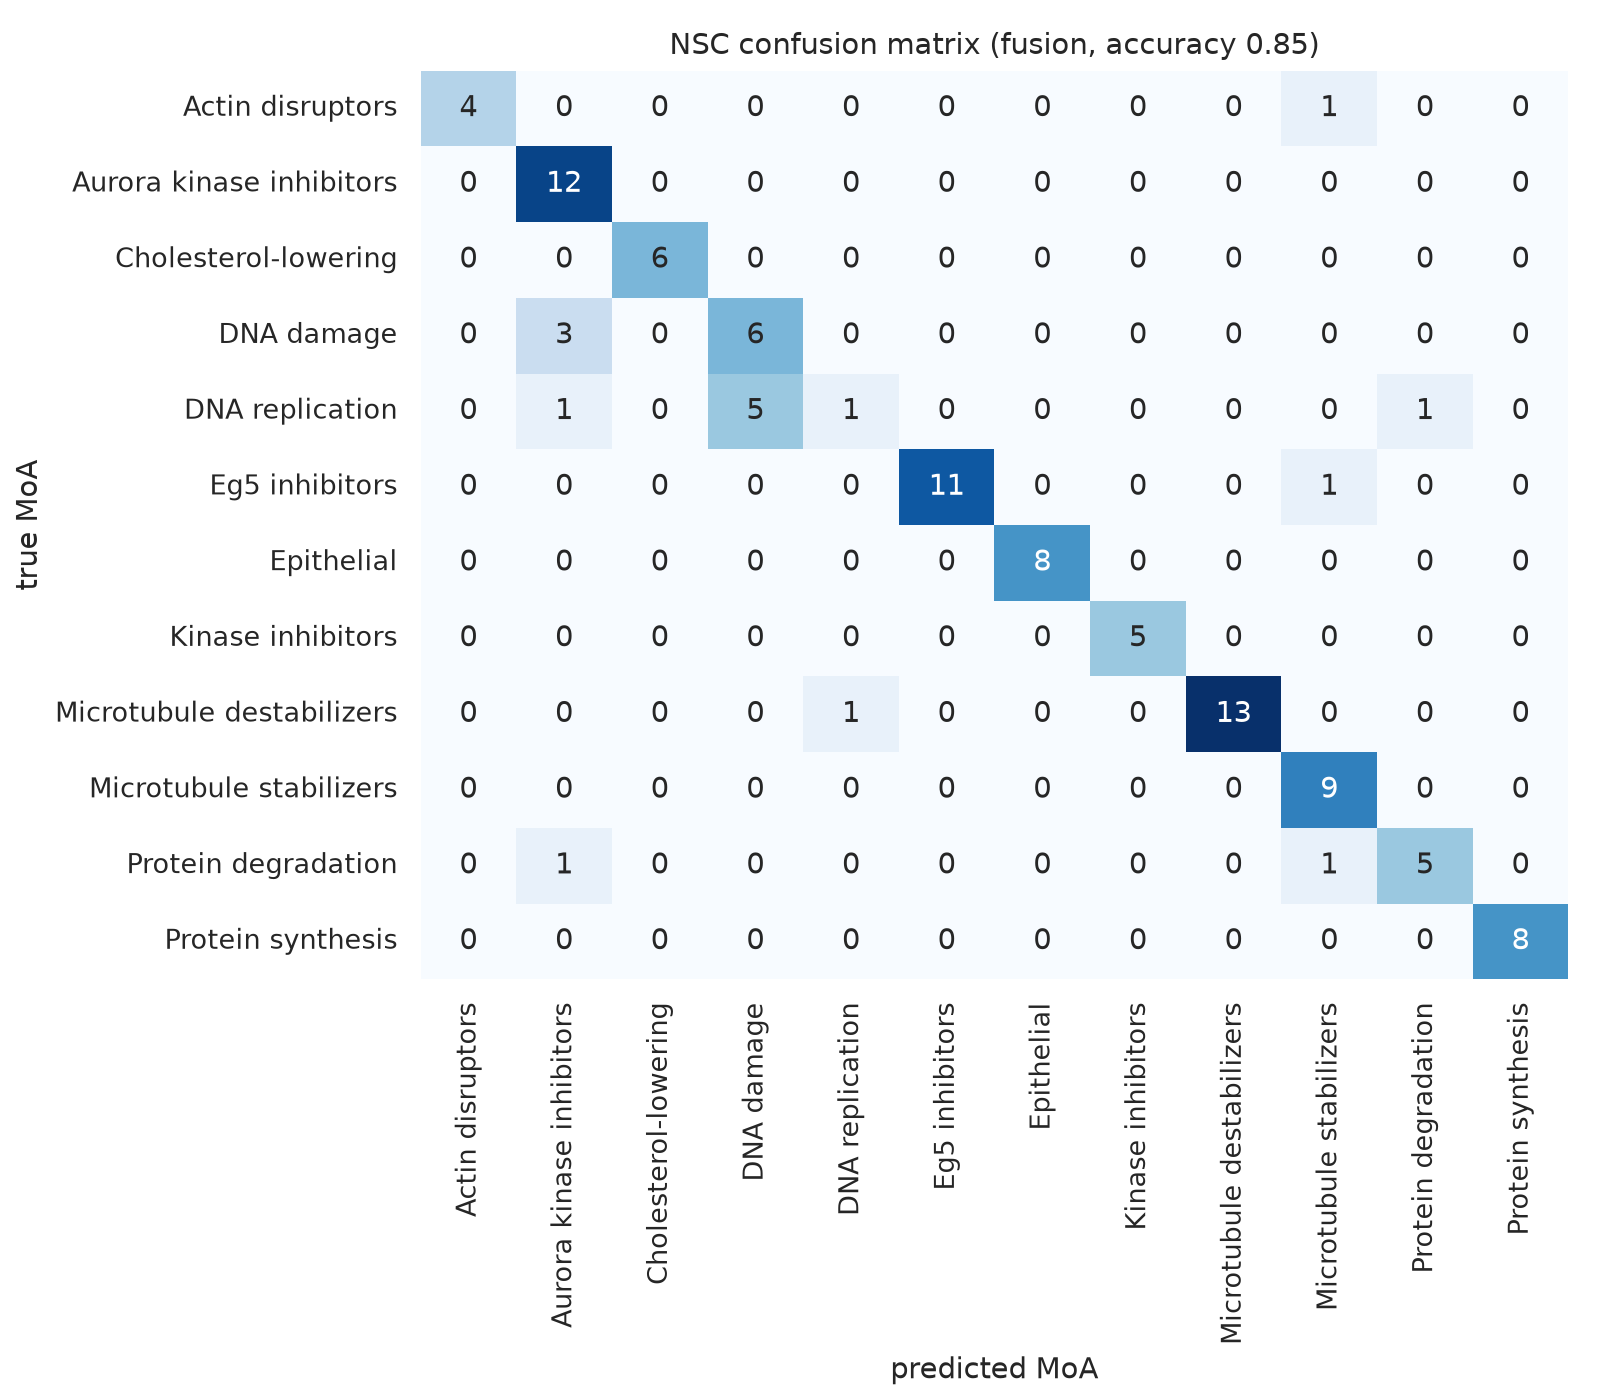
\includegraphics[width=0.48\linewidth]{fig_confusion.png}\hfill
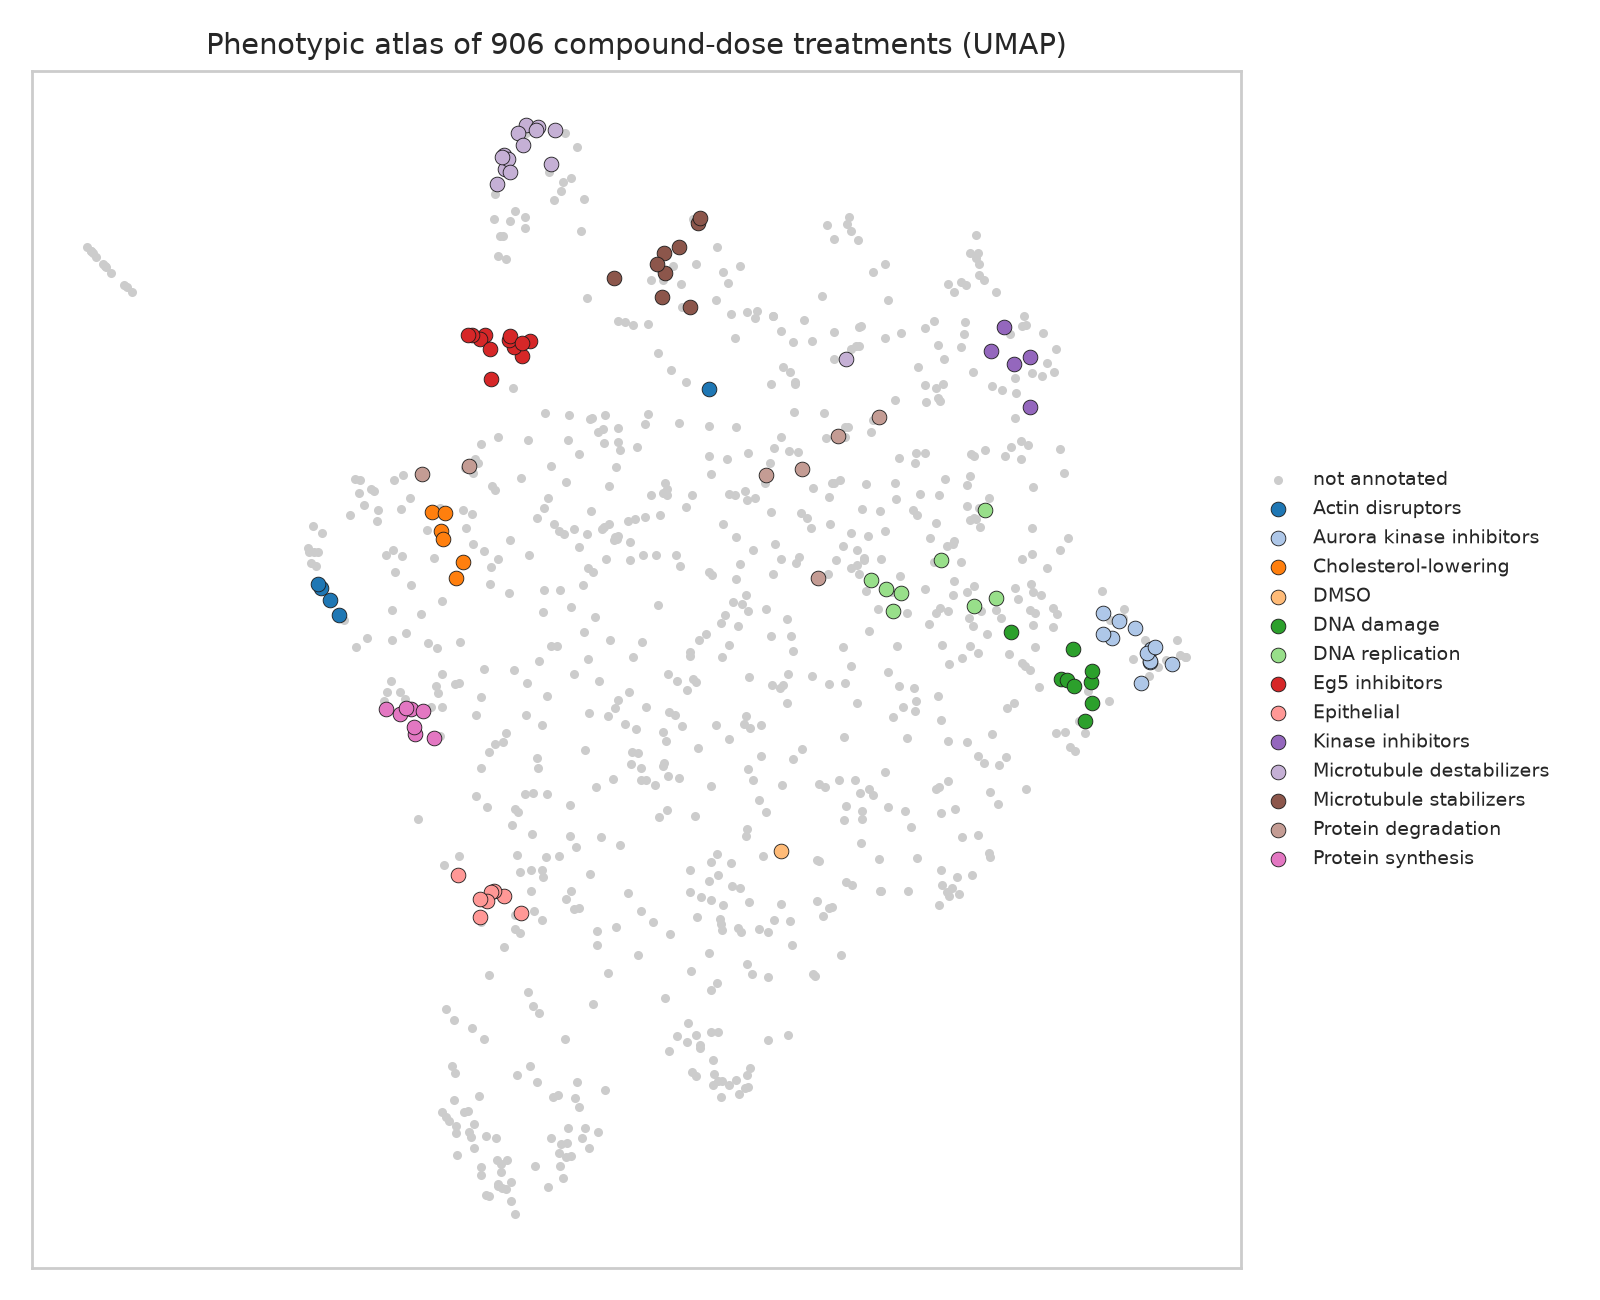
\includegraphics[width=0.5\linewidth]{fig_umap.png}
\caption{Left: NSC confusion matrix of the fusion profile. Right: UMAP of all 906
compound--dose treatments; grey points are the $\sim$800 un-annotated treatments, which Shennong's Glass
also places and labels.}
\end{figure}

\paragraph{Mechanisms the library was never told about.} About 800 of the 906 treatments carry
no MoA label. Among them, \emph{vinblastine} --- a vinca alkaloid and a classic cause of
chemotherapy-induced peripheral neuropathy~\cite{staff2017} --- is called a microtubule
destabiliser at 7 of its 8 doses, from 3\,nM, with probabilities 0.71--0.98; the unannotated
tubulin binder \emph{podophyllotoxin} receives the same call at its active dose. Calls made only
at overtly cytotoxic doses are less specific (e.g.\ camptothecin and mitomycin~C are labelled
microtubule-like at their top doses), which is why the triage reports the cytotoxicity window
alongside every mechanism call.

\subsection{Reliability}\label{sec:rel}
\begin{figure}[H]
\centering
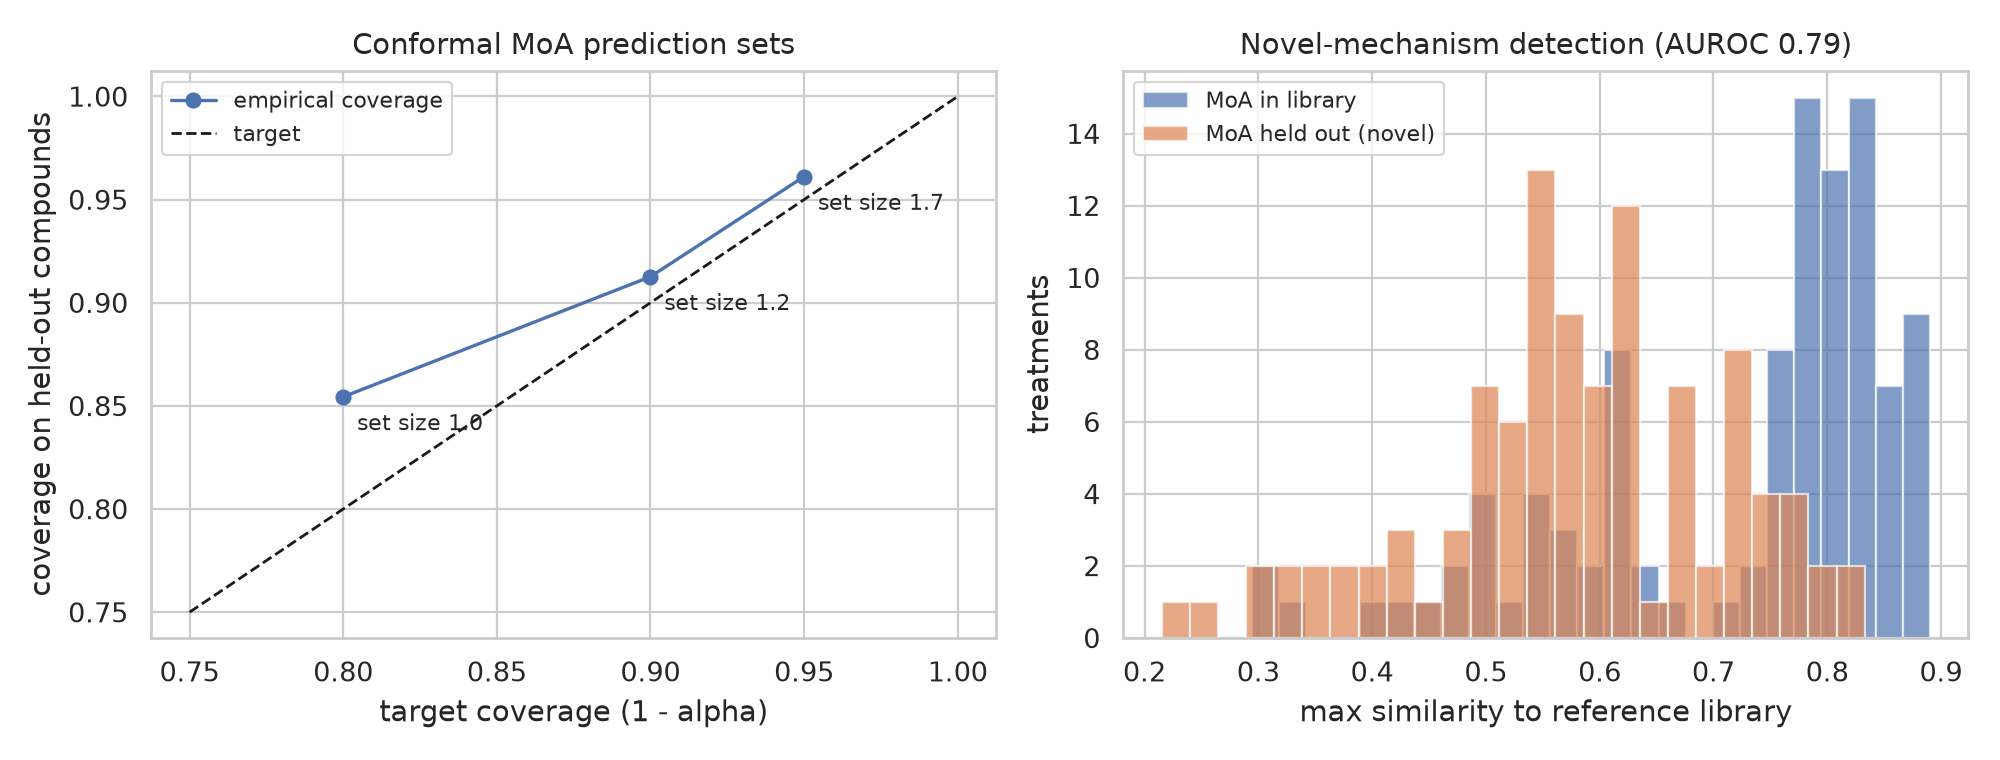
\includegraphics[width=0.9\linewidth]{fig_reliability.png}
\caption{Left: conformal coverage on held-out compounds versus target. Right: maximum similarity
to the library when the true MoA is present (blue) or hidden (orange).}
\label{fig:rel}
\end{figure}
Conformal sets meet their target: \CovNinetyFive{} coverage at 95\% (mean set size
\SizeNinetyFive), \CovNinety{} at 90\% (size \SizeNinety; \SingNinety{} of sets are single
MoAs) and \CovEighty{} at 80\% (size \SizeEighty). Hiding a query's own mechanism lowers its
best library similarity enough to be detected with AUROC \NoveltyAUROC{}. Finally,
\PctReplicatingAnn{} of the annotated (active) treatments have replicate wells more similar to
each other than the 95th percentile of random well pairs (\emph{percent replicating});
across all 906 treatments, including the many at sub-active doses that are not expected to
replicate, the figure is \PctReplicating.

\subsection{Dose--response and cytotoxicity window}
\begin{figure}[H]
\centering
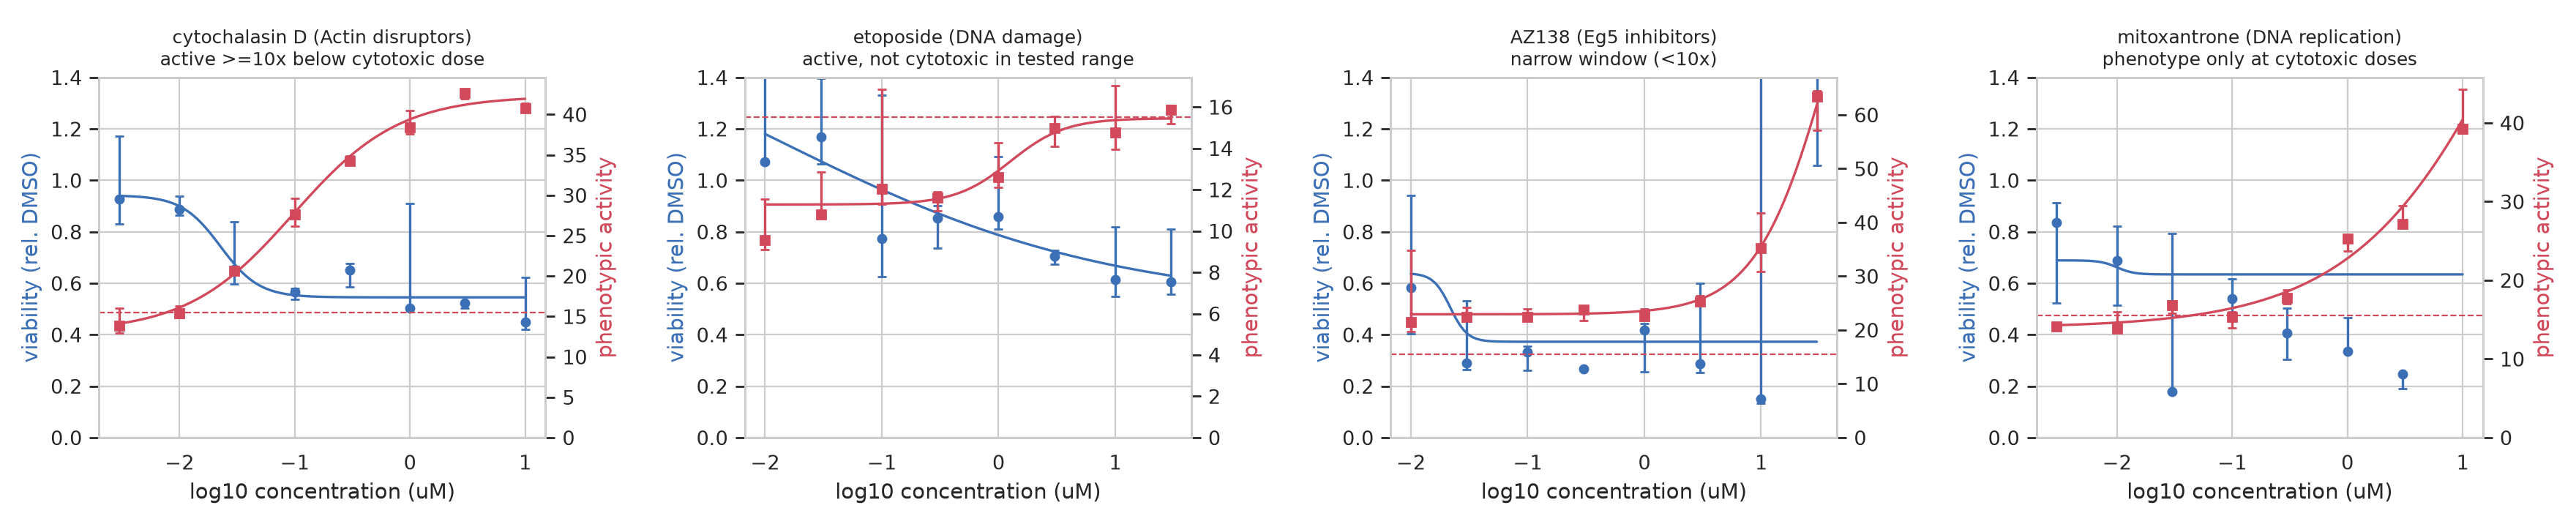
\includegraphics[width=\linewidth]{fig_dose_examples.png}
\caption{Viability (blue) and phenotypic activity (red; median and inter-quartile range over
wells; dashed line = 99th percentile of DMSO) with Hill fits, for one annotated compound of
each triage class (selected automatically: the most active compound of the class).}
\end{figure}
\begin{figure}[H]
\centering
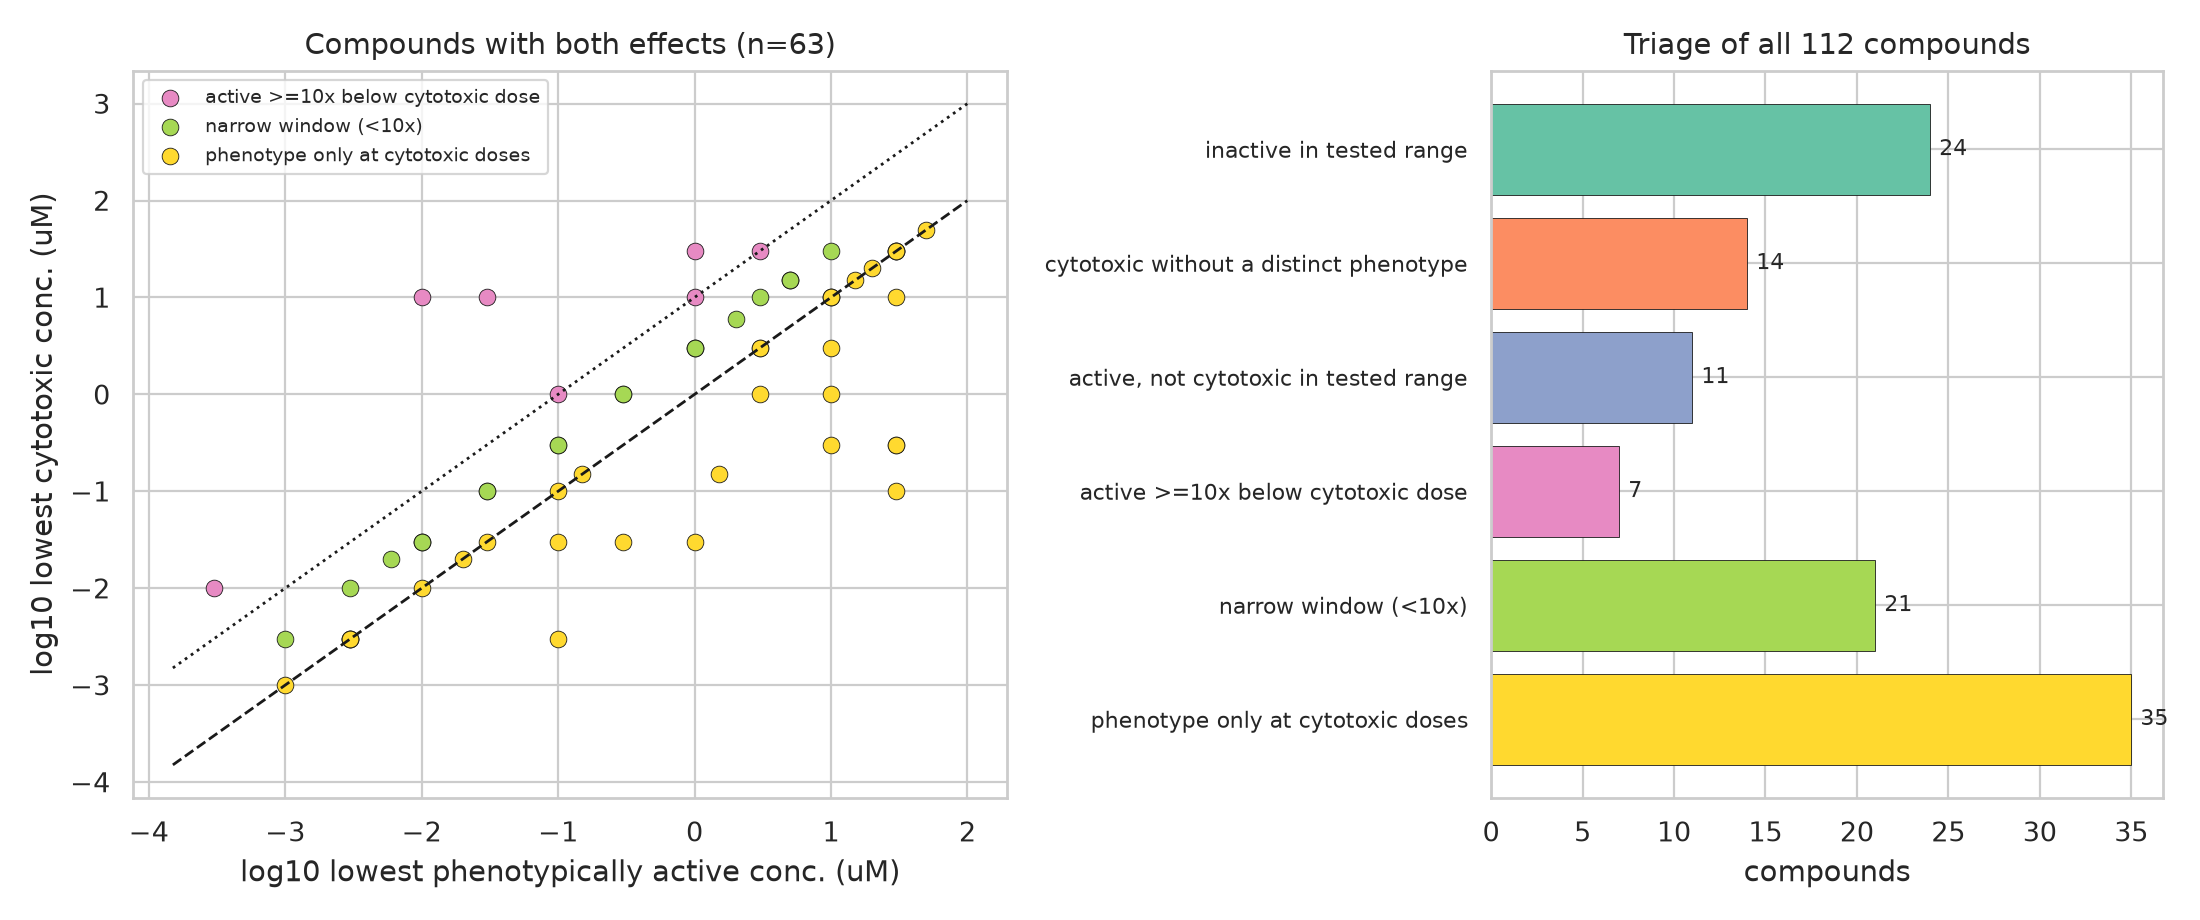
\includegraphics[width=\linewidth]{fig_window.png}
\caption{Left: lowest phenotypically active versus lowest cytotoxic concentration for the
compounds that show both (dashed: equal; dotted: $10\times$ window). Right: triage of all
compounds.}
\end{figure}
Of \NCompounds{} compounds, \NInactive{} show neither a phenotype nor cytotoxicity in the
tested range and \NToxOnly{} reduce cell number without a sustained specific phenotype;
\NNonTox{} are active without overt cytotoxicity, \NWideWindow{} act at least $10\times$ below
their cytotoxic dose, \NNarrow{} have a narrower window and \NToxFirst{} only change morphology
at doses that already reduce viability. This separation is exactly the information needed to
prioritise compounds --- or, for a
toxicity panel, to flag those whose cytoskeletal phenotype precedes cell loss.

\subsection{Interpretability}
\begin{figure}[H]
\centering
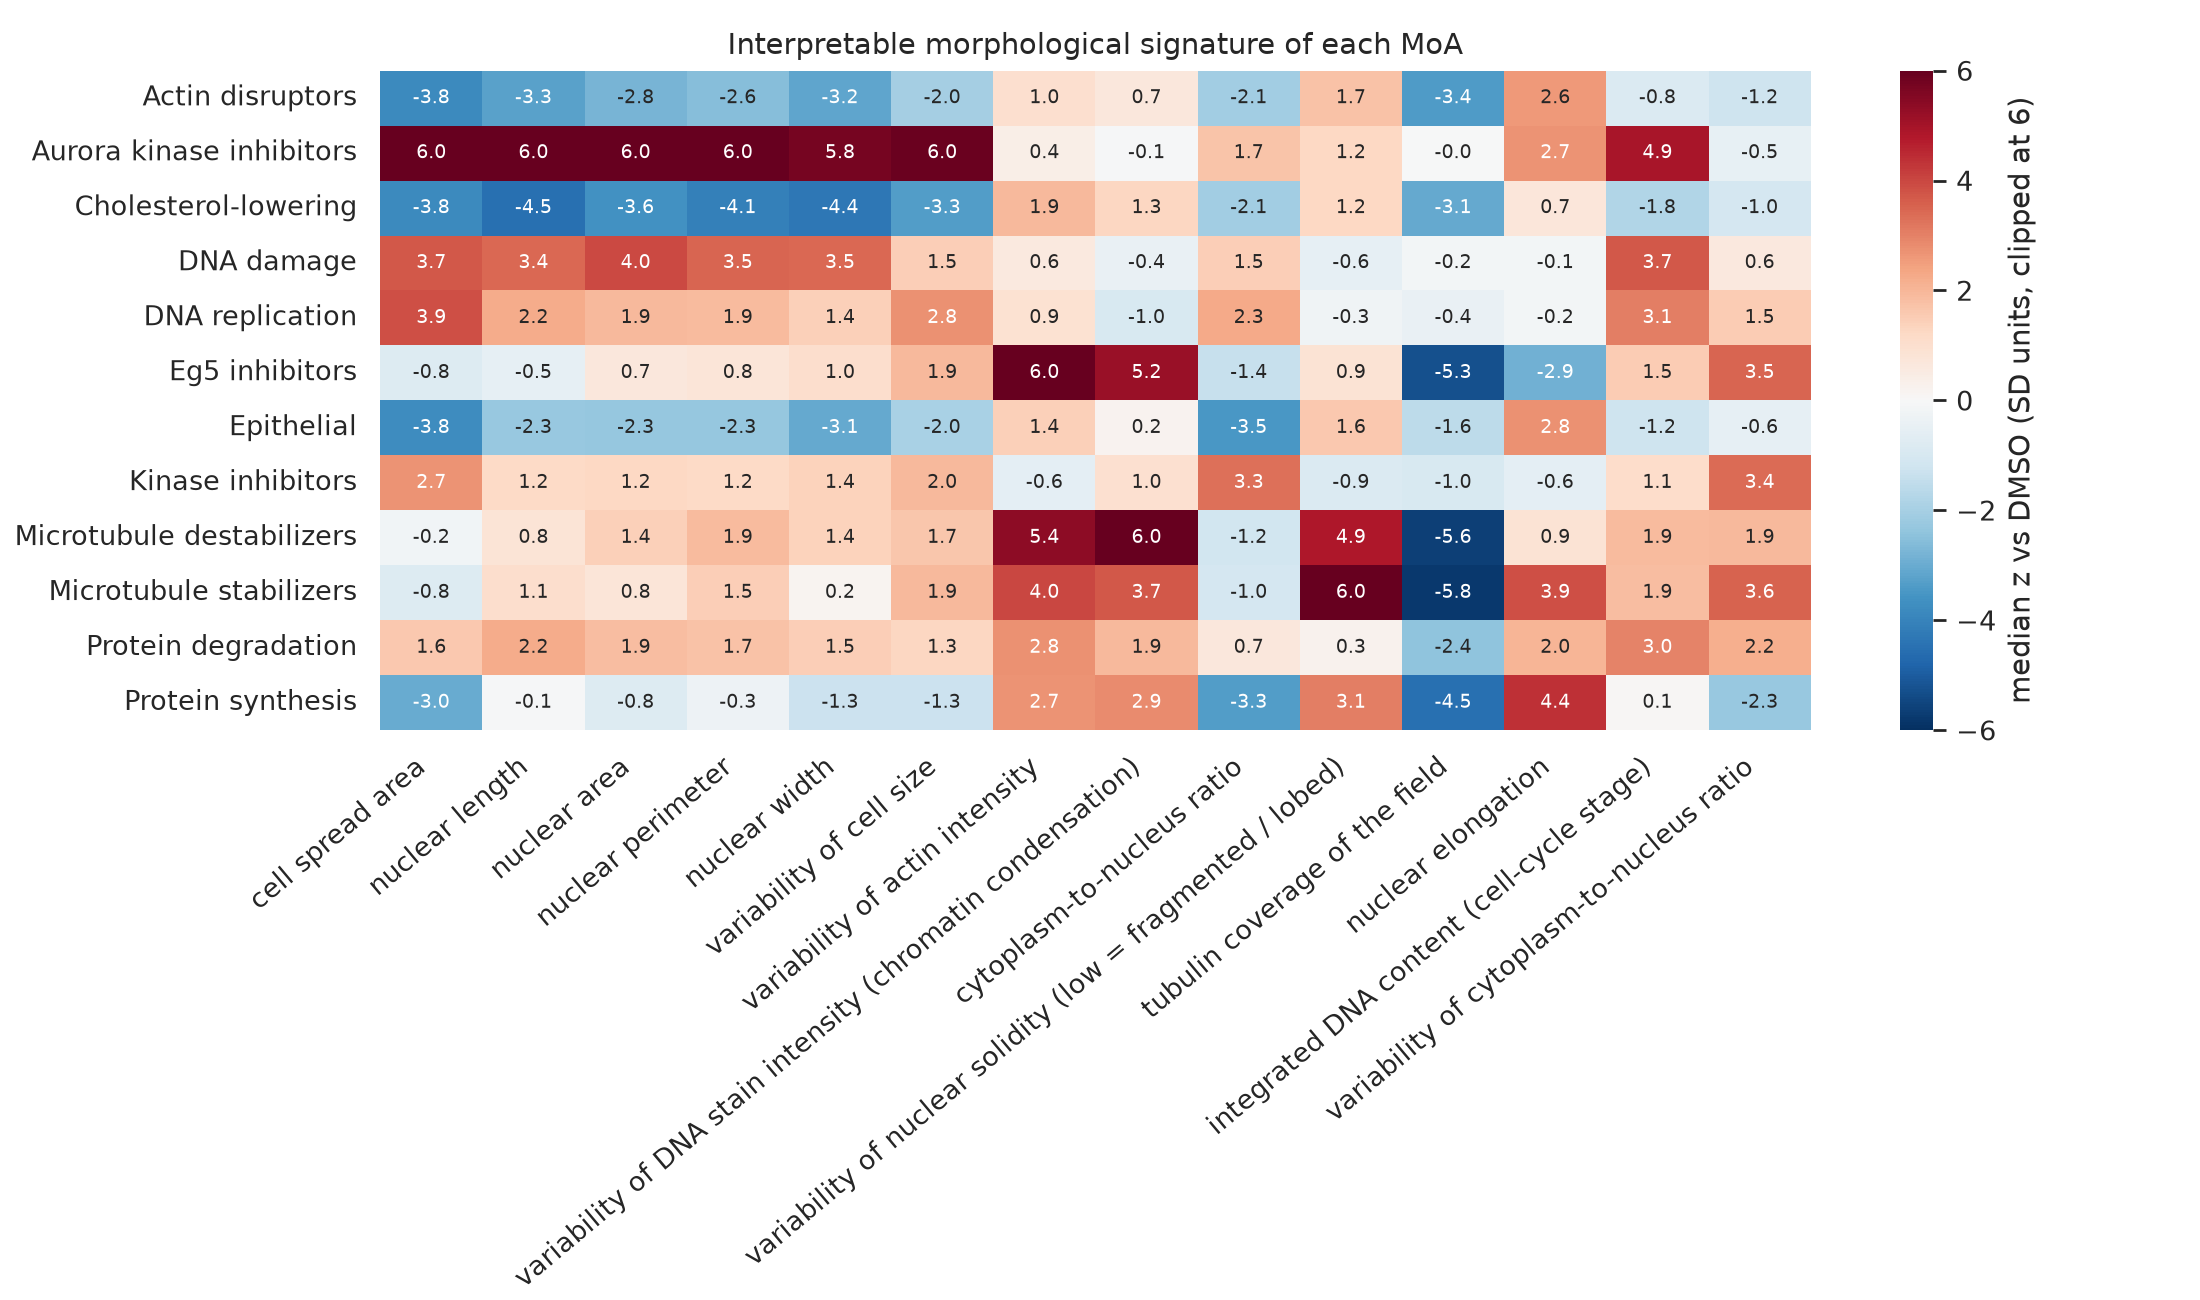
\includegraphics[width=0.85\linewidth]{fig_signatures.png}
\caption{Median morphological signature of each MoA ($z$ vs.\ DMSO in SD units; the 14 most
MoA-discriminative features). The signatures recover known biology without supervision:
Aurora-kinase inhibitors produce giant, DNA-rich nuclei (polyploidy after failed cytokinesis);
DNA-damaging and replication inhibitors enlarge nuclei and raise DNA content (S/G2 arrest);
Eg5 inhibitors and microtubule stabilisers/destabilisers increase the heterogeneity of DNA and
tubulin staining while reducing tubulin coverage (rounded mitotic cells with condensed
chromosomes); protein-synthesis inhibitors, actin disruptors and statins shrink cell spread area.}
\label{fig:sig}
\end{figure}

\section{Interactive system}\label{sec:demo}
The Gradio application has four tabs. \textbf{Analyze images}: upload the three channels of a
field; Shennong's Glass shows the segmentation overlay, the activity score with its percentile among
vehicle fields (active / borderline / inactive), the MoA ranking with 90\% conformal set when the
field is active, a novelty warning when appropriate, the morphological changes in words, and the
six most similar reference treatments with thumbnails. A
\emph{blind-test} switch removes a chosen compound from the library, so the bundled examples are
evaluated honestly. \textbf{Compound explorer}: dose--response, cytotoxicity window, dose-wise MoA
calls (suppressed at inactive doses) and representative images for every compound.
\textbf{Phenotypic atlas}: interactive UMAP of all 906 treatments. \textbf{Benchmark}: the
validation results above.

\section{Reliability analysis and limitations}\label{sec:limits}
\begin{itemize}
\item \textbf{Not yet OoC data.} BBBC021 is a 2D monolayer of one cancer line. The pipeline only
assumes the three stains, but 3D perfused chips add z-stacks, mixed cell types, PDMS
autofluorescence and channel geometry. The next step is to rebuild the reference library on chip
images (e.g.\ neural chips treated with reference neurotoxicants) --- no retraining is required,
but validation is.
\item \textbf{Reduced sampling.} Kaggle GPU sessions were unavailable while this work was done,
so features were extracted on CPU: 2 of 4 fields per well, 16 cells per field and the small ViT-S
encoder. One of the eight extraction shards did not finish in time, so \NImages{} of the 6{,}600
selected fields are used (every one of the \NWells{} wells retains at least one field). The full
configuration (ViT-B/14, 4 fields, 32 cells, all fields) is implemented in the same script and
is expected to improve the results; we do not claim that here.
\item \textbf{Viability proxy.} Cell count after 24\,h conflates cytostatic and cytotoxic effects
and is sensitive to seeding density. At the most toxic doses apoptotic nuclei fragment and are
over-counted, occasionally pushing ``viability'' above 1; Hill fits therefore use a robust
(soft-$\ell_1$) loss. Dedicated viability stains or LDH release would be better.
\item \textbf{Conformal guarantee is marginal} and assumes compounds are exchangeable with the
reference set; coverage for structurally novel chemotypes may be lower, which the novelty flag
partly mitigates.
\item \textbf{Single-field uploads} are normalised against global rather than plate-matched DMSO
statistics and are therefore noisier than plate-level analysis. The demo calibrates its activity
percentile on single DMSO fields, reports borderline fields (80th--95th percentile) as
low-confidence, and withholds mechanism calls below that; the conformal coverage guarantee
applies to treatment-level profiles and is optimistic for a single field. In our bundled
examples, a single colchicine field is flagged as borderline and receives a wrong mechanism ---
exactly the case the low-confidence warning is meant to catch.
\item \textbf{Segmentation} is classical and tuned for MCF-7 nuclei; dense 3D tissue would need a
learned segmenter (e.g.\ Cellpose).
\end{itemize}

\section{Potential impact}
Because Shennong's Glass needs no training, a lab can deploy it on a new chip in a day: image a few dozen
reference compounds with known mechanisms and vehicle controls, and every subsequent compound
gets an MoA hypothesis with calibrated confidence, a potency/toxicity window and an
explanation. Calibrated sets and novelty flags make it safe to use for triage: ambiguous or
unprecedented phenotypes are routed to experts instead of silently mislabelled. For neural OoC in
particular, the tubulin/actin read-outs at the core of the method are the ones that report
axonal and cytoskeletal toxicity, making it a candidate early-warning system for
neurotoxic liabilities such as those of microtubule-targeting chemotherapies. We see this as a
step towards the data-driven ``digital twin'' of a chip assay: a reusable, quantitative,
uncertainty-aware map from images to pharmacology.

\section{Reproduction}
\begin{verbatim}
pip install -r requirements.txt            # CPU is enough
kaggle auth login                          # free account
bash scripts/fetch_data.sh                 # metadata, features, example images
python scripts/run_analysis.py             # results/ + artifacts/  (< 1 min)
python app/app.py                          # http://127.0.0.1:7860
\end{verbatim}
Raw-image feature extraction: run \texttt{kaggle/features/features.py} (or the sharded CPU
variants in \texttt{kaggle/cpu\_shards/}) as Kaggle notebooks with dataset
\texttt{stanleyhua/bbbc021} attached, then \texttt{scripts/merge\_features.py}.

\section*{Team}
\TeamDetails

\begin{thebibliography}{99}\small
\bibitem{caie2010} P.~D. Caie et al. High-content phenotypic profiling of drug response signatures across distinct cancer cells. \emph{Mol. Cancer Ther.} 9(6):1913--1926, 2010.
\bibitem{ljosa2012} V.~Ljosa, K.~L. Sokolnicki, A.~E. Carpenter. Annotated high-throughput microscopy image sets for validation. \emph{Nat. Methods} 9:637, 2012.
\bibitem{ljosa2013} V.~Ljosa et al. Comparison of methods for image-based profiling of cellular morphological responses to small-molecule treatment. \emph{J. Biomol. Screen.} 18(10):1321--1329, 2013.
\bibitem{ando2017} D.~M. Ando, C.~Y. McLean, M.~Berndl. Improving phenotypic measurements in high-content imaging screens. \emph{bioRxiv} 161422, 2017.
\bibitem{oquab2023} M.~Oquab et al. DINOv2: Learning robust visual features without supervision. \emph{Trans. Mach. Learn. Res.}, 2024 (arXiv:2304.07193).
\bibitem{vovk2005} V.~Vovk, A.~Gammerman, G.~Shafer. \emph{Algorithmic Learning in a Random World}. Springer, 2005.
\bibitem{angelopoulos2021} A.~N. Angelopoulos, S.~Bates. A gentle introduction to conformal prediction and distribution-free uncertainty quantification. arXiv:2107.07511, 2021.
\bibitem{ingber2022} D.~E. Ingber. Human organs-on-chips for disease modelling, drug development and personalized medicine. \emph{Nat. Rev. Genet.} 23:467--491, 2022.
\bibitem{low2021} L.~A. Low, C.~Mummery, B.~R. Berridge, C.~P. Austin, D.~A. Tagle. Organs-on-chips: into the next decade. \emph{Nat. Rev. Drug Discov.} 20:345--361, 2021.
\bibitem{staff2017} N.~P. Staff, A.~Grisold, W.~Grisold, A.~J. Windebank. Chemotherapy-induced peripheral neuropathy: a current review. \emph{Ann. Neurol.} 81(6):772--781, 2017.
\end{thebibliography}
\end{document}
